% Chapter 1
% 
\chapter{Introduction} % Main chapter title
\label{chap:Chapter1} % For referencing the chapter elsewhere, use Chapter~\ref{Chapter1}


%-------------------------------------------------------------------------------
%---------
%
\section{Overview}
\label{sec:chap1_guidelines} %For referencing this section elsewhere, use Section~\ref{sec:chap1_guidelines}
Since the discovery of electricity, humanity has harnessed electrical energy for a multitude of purposes. As the demand for electricity grew, encompassing applications like heating, ventilation, and lighting, the need to generate more electrical power became paramount to accommodate the evolving array of functionalities that emerged over time.

Consequently, diverse power plants were established to meet the increasing demand. These included thermal power plants, hydroelectric plants, nuclear facilities, geothermal installations, combined-cycle plants, and others. In contemporary times, we have witnessed the advent of novel energy sources, such as wind, solar, tidal, biomass, and green hydrogen. Classified as renewable energies, these sources, along with hydroelectric power, offer a pathway towards planetary decarbonization, as they eschew reliance on fossil fuels.

However, these power-generating facilities often found themselves situated at a considerable distance from major consumers, specifically large urban centers. This spatial disparity necessitated the development of a means to efficiently transport the energy generated by these plants to the significant consumer hubs. This necessity gave rise to electrical substations, pivotal in facilitating the transmission of energy from power plants to end consumers, thereby playing a fundamental role in the entire energy cycle.

However, the introduction of electrical substations takes place, and while various types exist,here spotlight four specific substation categories here:

\begin{itemize}
	\item Step-up substations: Positioned in close proximity to power plants, these substations serve the crucial function of elevating the energy voltage. This strategic placement aims to minimize losses attributable to phenomena such as Foucault currents and parasitic currents, ensuring the delivery of generated power with utmost efficiency. Given the substantial distances involved in transmission, the decision to increase voltage at this stage becomes imperative to effectively mitigate the mentioned challenges.
	
	\item Distribution Substation: Following the transmission of energy from remote areas at higher voltages to minimize losses, it becomes essential to lower the voltage before reaching consumers at safer levels. This leads to distribution substations, where the voltage is reduced, allowing for a more seamless distribution of energy within urban centers.
	
	\item Step-Down Substation: The step-down substation is the one located very close to the end consumer, operating at a lower voltage than in distribution, thereby reducing the risks to the individuals who utilize it.
	
	\item Switching Substation: This facility is designed to interconnect supply circuits operating at the same voltage level. It allows for the segmentation of circuits, facilitating the power on of shorter sections, and enabling a more flexible and efficient distribution of electrical power.
	
\end{itemize}

Figure~\ref{fig:electricity-pathway} is a diagram illustrating the path from the power plant where the energy is generated, going through high power transformer to elevate the voltage to have minimum losses, the transmission line to transmit all the power, a high power transformer to step down the voltage and send the energy to the end consumer,~\footnote{\url{https://www.eia.gov/energyexplained/electricity/delivery-to-consumers.php}}.

\begin{figure}[tbh!]
	\centering
	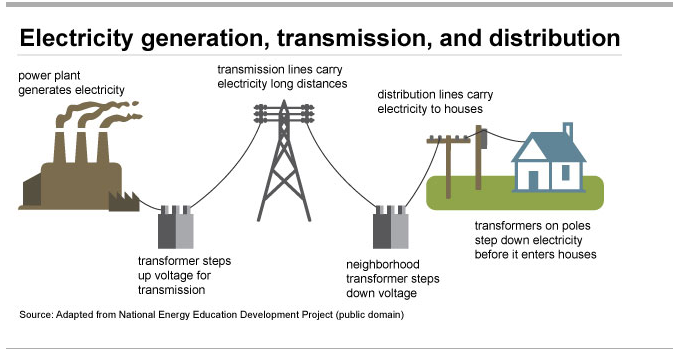
\includegraphics[width=\textwidth, keepaspectratio]{ch1/assets/Way_of_electricity.png}
	\caption{Electricity Generation, Transmission, and Distribution Pathway (Image credits: U.S. Energy Information Administration)}
	\label{fig:electricity-pathway}
\end{figure}

\section{Digital Substation}
Electric power substations play a fundamental role in the entire cycle of electric energy and its transformations. Simultaneously, as we witness several generating sources converting energy, such as hydroelectric (water turbines), thermal (steam turbines), combined cycle (gas turbines and steam turbines), wind (wind energy), solar farms (solar energy), among others into electric energy, numerous consumers draw upon this produced energy. The absence of an energy storage location underscores the substantial importance of substations. Without them, meeting the extensive demand and need for electric energy would be impracticable, hindering economic growth and the development of industries, businesses, and even entire countries. Today, every facet of operation, from mega-factories to simple light bulbs, relies on electric energy.

Substations facilitate the extended reach of energy to diverse locations, enabling a direct connection from the generating source to consumers. Serving as the link between generation and consumption, substations categorize the electric energy chain into four major divisions: electric energy generation, electric energy transmission, electric energy distribution, and electric energy consumption. These processes start with High Voltage (Generation), increases to Very High Voltage (Transmission), goes to Medium Voltage (Distribution) and when finally reaches the consumer is Low Voltage (Consumers).

The evolution of electric substations has embraced new technologies, as preventive maintenance, predictability of problem occurrences, fault alerts, backyard equipment switching, and visualization of currents and voltages. Follow these advancements are electromechanical protection relays, monitoring and safeguarding against electrical faults in backyard equipment.
Backyard equipment, including high-voltage circuit breakers, switches, capacitor banks, reactors, transformers, and transmission lines, retains the basic concept from the 1990s but now has features enhanced performance and added functionalities due to technological advances.

Electric power systems within a substation can be categorized into four levels:

\begin{itemize}
	\item Level 0 - Backyard Equipment: Encompassing all devices responsible for transmitting energy from the power generation station to customers, factories, public lighting, residences, hospitals, data centers, etc. These devices are responsible for the entire energy system.
	\item Level 1 - Protection Relays: Formerly known as Intelligent Electronic Devices (IED), these devices have replaced the need for multiple protection relays, executing a lot of protection functions, such as overcurrent, overvoltage and transformer differential, within a single device and add the communications possibilities, exchange information between devices.
	\item Level 2 - Supervisory Control and Data Acquisition (SCADA): SCADA systems communicate with IEDs to acquire data, including readings of currents and voltages, facilitating the supervision of the entire substation and remote operation of backyard equipment.
	\item Level 3 - Control Center: This centralizes information from multiple substations, commanding them in a manner conducive to the grid and handling functions inherent to Level 2. Typically used by those overseeing the distribution of electrical energy system throughout a country, it ensures a balanced load throughout varying consumption periods.
\end{itemize}

Over the years, substations have evolved to the concept of a digital substation. Even today, it is a very current topic, we moved from having less 'smart' equipment to having every device becoming more 'smart'.

The concept of a digital substation involves seamless communication between devices across all levels, minimizing the need for electrical wires and favoring optical fiber as the primary means of information exchange. Devices communicate with each other, enabling actions such as a trip originating from an IED communicating with a circuit breaker via the network to address a fault identified by the IED. This is achieved through a message called Generic Object-Oriented Substation Event (GOOSE), and the circuit breaker itself triggers the operation through the GOOSE protocol, exemplifying the digital substation concept. While the world still faces limitations in fully embracing the digital substation concept, notable progress has been made at Level 0, particularly with the introduction of Merging Units (MU). These units perform analog acquisition of current and voltage sensor data and inform other devices digitally on the network.

This marks another step towards the digital substation concept, where only this equipment is connected to the sensors, and a single optical fiber connects to a switch to publish information from the respective sensors. Today, there is no longer a need to connect wires to the electrical protection panel, connect the IEDs to the same network as the Merging Unit provides the necessary information to execute electrical protection algorithms.

\section{Research Motivation and Context}
With the advent of the IEC~61850 standard in the energy sector, emerging as the definitive standard for the entire industry, facilitating essential interoperability among diverse equipment from various manufacturers, ensuring reliability, real-time responsiveness, and resilience over time. Fueled by a deep passion for the field of electrical energy.

Presently, It is actively contributed to the improve of IEDs, developing a solution wherein the device possesses decision-making capabilities. This involves choosing, through the IEC 61850-9-2 Samples Values protocol, which sample provided by the Merging Units to employ in the algorithms of the protection device.

This endeavor allows me to amalgamate my extensive experience in commissioning electrical substations, particularly in conducting primary and secondary tests with a focused emphasis on secondary evaluations.

The insights gained from my pursuit of a Master's degree in Critical Computing Systems are seamlessly integrated into this tangible development. The aim is to enhance a critical functionality of IEDs, positioning these devices as the cornerstone with the most critical actuation power within an electrical substation. This commitment ensures optimal response times while steadfastly adhering to the foundational principles of electrical protections and the four pillars of electrical protection:

\begin{itemize}
	\item Reliability: The likelihood of a component, equipment, or system meeting its intended function under specified circumstances, while avoiding unnecessary operations during routine system operation or in the presence of faults outside its protection zone.
	\item Sensitivity: The capacity of the protection system to respond to abnormalities in the designated operating conditions, selectively isolating only the portion of the system experiencing a fault, while allowing the rest to operate normally.
	\item Selectivity: The ability to completely isolate the faulty element and disconnect the smallest possible portion of the system by operating associated breakers.
	\item Speed: The commitment to minimizing the impact of faults and the risk of instability, quantified by the time between fault occurrence and the opening command of the circuit breaker issued by the relay or IED.
\end{itemize}

\section{Research Objectives}

The ongoing digital transformation of electrical substations has led to the development of a crucial component known as the Merging Unit. This advanced equipment plays a significant role in modernizing substations by enabling the acquisition of data from current and voltage transformers. Its main function is to read and process these values and then transmit them via the IEC~61850-9-2 Sampled Values (SV) protocol.

A scenario may occur in which two Merging Units simultaneously read data from the same current or voltage transformer. Both units independently send Sampled Values over the Ethernet network, creating a need for a decision-making mechanism within the IED. The IED, which is a key element in protection systems, must possess the capability to identify and select the optimal sample for use in its protection algorithms.

This research focuses on developing the intelligence required for the IED to autonomously evaluate and choose between the multiple samples provided by the Merging Units. By improving the decision-making abilities of the IED, the research aims to optimize the performance and reliability of protection systems in digital substations, ultimately enhancing the overall efficiency and resilience of the power grid.

\section{Research Contributions}
This thesis introduces a significant contribution through the proposition of an algorithm designed to optimize the selection of samples from each current transformer and voltage transformer for individual electrical protection relays. These algorithms are instrumental in ensuring that electrical protection systems adhere to the four key principles of protection philosophy. Recognizing that the same Merging Unit may not yield optimal results for all protection relays, the effectiveness of the algorithm is contingent on various factors, including communication routes, the distance information travels, and potential network issues such as information overload, given the abundance of sampled values in the network. As such, the primary contribution of this thesis lies in the development of an algorithm capable of discerning the most suitable sample for consumption by the IED in the network.

This work also investigates the use of the Rust programming language to facilitate communication using the IEC~61850 standard.
In the absence of a Rust library for this purpose, we developed custom functions to pack and unpack SV into IEC~61850 packets.
The source code is openly available at \url{https://github.com/everton-oriente/IEC61850_9_2_SV} and can be integrated into other projects or compiled for any platform supported by Rust.


\section{Thesis Structure}

The current thesis is organized into seven sections: Introduction, State of the Art, Research Topic, Implementation, Development of the Algorithm, Tests and Evaluation, and Conclusions. Together, these chapters comprehensively cover all aspects of the topic, ensuring a thorough exploration and analysis within the scope of this master's thesis.

In Chapter 2 - Background on Substation Automation: This chapter reviews the existing literature and technologies related to substation automation systems, with a focus on digital substations. It provides a detailed analysis of various components such as circuit breakers, switches, and transformers, as well as the role of Intelligent Electronic Devices (IEDs) in protection, control, measurement, and monitoring. The chapter also delves into the IEC 61850 standard, explaining its different parts and their significance in modern substation communication protocols.

In Chapter 3 - Analysis and Design of the Solution: This chapter explores the specific research problem addressed in the thesis. It identifies the research gap by analyzing existing literature and related studies, discussing why addressing this gap is important. The chapter outlines the architecture of the algorithm developed to solve the identified problem, setting the groundwork for the implementation and testing described in subsequent chapters.

In Chapter 4 - Architecture: This chapter details the practical aspects of developing the proposed algorithm. It covers the hardware and software components used, including specific technologies and tools such as Rust crates. The chapter explains how the algorithm was developed, including the selection of sampled values  and the overall architecture. It also discusses the challenges faced during implementation and how they were overcome.

In Chapter 5 - Implementation: This chapter focuses on the detailed development process of the algorithm for IEC 61850-9-2-SV. It explains the structure of sampled values, the creation of a publisher and subscriber for SVs, and the core functions of the algorithm. The chapter also discusses the simulation of electrical grid signals and the introduction of invalid samples for testing purposes. The finalization of both the publisher and subscriber is covered, along with the overall development of the algorithm.

In Chapter 6 - Tests and Evaluation: This chapter presents the testing and evaluation of the developed algorithm. It includes detailed tests of the publisher and subscriber for IEC 61850-9-2-SV, as well as the overall algorithm's performance. The chapter discusses the results of these tests, evaluating the algorithm's effectiveness in meeting the research objectives and its potential for real-world application.

In Chapter 7 - Conclusion: The final chapter summarizes the thesis, discussing the limitations of the research and the conclusions drawn from the study. It also offers suggestions for future work, including potential improvements to the algorithm, the addition of new features, and the exploration of further research opportunities in digital substations and related technologies.
